\documentclass[a4paper, 12pt]{report}

\usepackage{graphicx}

\begin{document}

% Title
\title{Second assignment documentation}
% Author
\author{Le Minh Nghia - AAOGMU}
\maketitle
\pagenumbering{Roman}
% Table of contents:
\tableofcontents

%CHAPTER:
\chapter{Assignment's description}
\pagenumbering{arabic}
	Create a game, which is a variant of the well-known five-in-a-row game. The two players can play on
a board consists of n x n fields. Players put their signs alternately (X and O) on the board. A sign can
be put only onto a free field. The game ends, when the board is full, or a player won by having five
adjacent signs in a row, column or diagonal. The program should show during the game who turns.

The trick in this variant is that if a player makes 3 adjacent signs (in a row, column or diagonal), then
one of his signs is removed randomly (not necessary from this 3 signs). Similar happens, when the
player makes 4 adjacent signs, but in this case two of his signs are removed.

Implement this game, and let the board size be selectable (6x6, 10x10, 14x14). The game should
recognize if it is ended, and it has to show in a message box which player won (if the game is not
ended with draw), and automatically begin a new game.

%CHAPTER:
\chapter{Usage}

Go to "out/production/Caro/" and call cmd, then run "java Main".

%CHAPTER:
\chapter{UML Diagram}
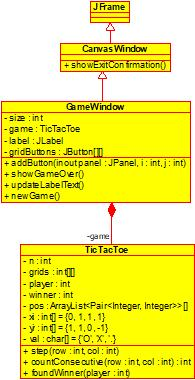
\includegraphics[scale=1.0]{class_diagram.jpeg}

%CHAPTER:
\chapter{Methods documentation}
\begin{itemize}
\item \textbf{CanvasWindow's methods:}
		\begin{description}
			\item[Constructor] Create a canvas frame with given size and one close event.
			\item[showExitConfirmation] Specify what will happen when clicking on the exit button.
		\end{description}
\item \textbf{GameWindow's methods:}
		\begin{description}
			\item[Constructor] Create a game window with the grids, buttons to choose size of grid, and label to show current player
			\item[addButton] Add new button at position (i, j) with event handler.
			\item[showGameOver] Show the winner and restart the game.
			\item[updateLabelText] Show who turns.
			\item[newGame] create new game.
		\end{description}
%\newpage
\item \textbf{TicTacToe's methods:}
		\begin{description}
			\item[step] Simulate 1 turn when a player clicked on cell (i, j). It then get the longest consecutive sequence which contains cell (i, j), after that, depends on that value \{3, 4, 5\}, the method will delete 1 random cell, 2 random cells, or end the game. The method will return a list of deleted position for display purpose.
			\item[countConsecutive] return the longest consecutive sequence in which cell (i, j).
			\item[isValid] check if cell (x, y) is belonged to the grids.
		\end{description}
\end{itemize}
%CHAPTER:
\chapter{Events and event handlers connection}
\begin{description}
	\item[Exit] Will be called when clicked on the close button.
	\item[Put \{X, O\} into the boards] Cell (i, j) will display \{X, O\} if a player clicked on it when it was empty.
	\item[Delete random] Happens when one player has 3 or 4 adjacent signs.
\end{description}

\end{document}

